\section{Background}
%%\todoalex{Comment by Alex}
%%\todomichael{Comment by Michael}
%%\todosanne{Comment by Sanne}
% First paragraph
In the era of big data and big science, \emph{computational reproducibility} is an important means to verify the validity of scientific conclusions drawn from raw data, and promotes \emph{reuse} of the research and its methods in downstream analyses. However, across multiple domains of science, computational reproducibility is often not achieved due to lack of transparency or \emph{code rot} \cite{committeeonreproducibilityandreplicabilityinscienceReproducibilityReplicabilityScience2019}. Given the prominent role which science plays in our society, this is a serious and challenging problem. Manually collecting all the information required for reproducibility is tedious, %Manually documenting the steps which led to a particular result is infeasible in practice, 
since current data analysis requires complex computational processes which use large datasets from many different sources, comprise various software tools, and are often executed on various computational systems many times as the methods are refined. Solutions which automate the recording of \emph{provenance} are therefore in high demand.
%For this reason, there is an urgent need for solutions which automate the recording of \emph{provenance}, i.e. all the steps which led to a particular result.
\begin{figure*}[!hb]
    \centering
    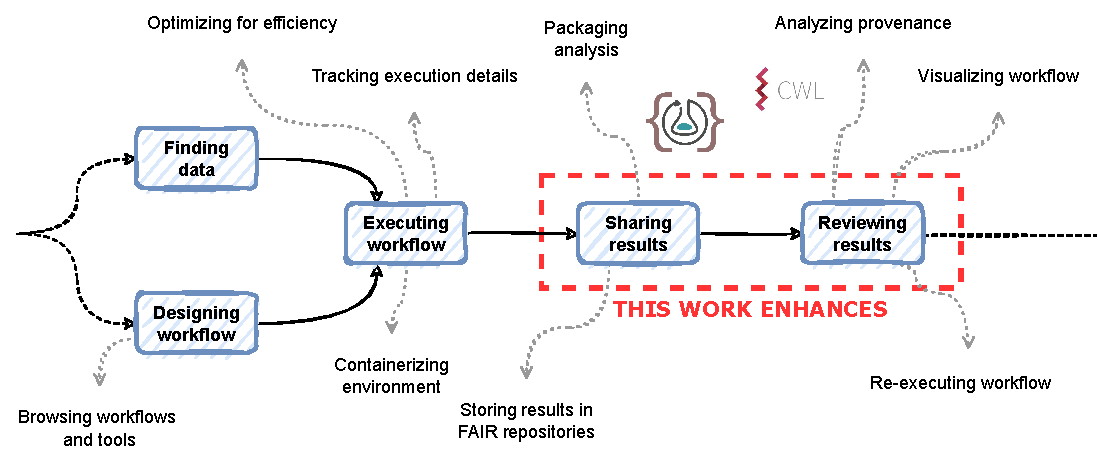
\includegraphics[width=1\textwidth]{background/vision.pdf}
    \caption{A vision of an ecosystem of workflow-related resources and its benefits for the reproducibility of computational processes. In this vision, workflows and data are stored in FAIR repositories, are executed in containerized environments by workflow systems which leverage efficient job-scheduling technologies and track details of the computation.  
    After publication, the results of the workflow can be analyzed, and workflows can optionally be re-executed as the start of new projects which build upon the research. 
    Fundamental to the success of this approach is the interoperability of the components of the ecosystem. In this work, we focus on workflow-centric Research Objects as a common format for the sharing and analysis of computational results.
    %\todorenske{Keep CWL(Prov) and ROCrate logos in?}
    }
    \label{fig:vision}
\end{figure*}
The transparency of computational analyses can be improved by expressing scientific analyses as \emph{workflows}, i.e. a series of steps with the output of one step becoming the input for another. Figure \ref{fig:vision} envisions a future in which workflows are an integral part of reproducible computational research, central to an ecosystem of tools and platforms which have emerged over the last decade. 
A crucial requirement to the success of this approach is that the workflow-related tools are compatible with each other, i.e. \emph{interoperable}. 

The problem of workflow interoperability has been partly addressed by the specification of Common Workflow Language (CWL) \citep{crusoeMethodsIncludedStandardizing2022}, a platform-neutral standard for workflow descriptions. CWL workflows are \emph{portable} across multiple workflow management systems. However, provenance of a computational result comprises more than a workflow description alone,
% a workflow description alone does not comprise the full provenance of a computational result, 
since the output data are also strongly dependent on the input configurations (data and parameter settings) and the (distributed) computational system(s) on which the workflow was executed. 


%%\stodor{Append CWLProv paragraph to wf-centric RO or separate paragraphs?} 
For this reason, workflow-centric \emph{Research Objects} (ROs) \cite{belhajjameWorkflowcentricResearchObjects2012} have been proposed as a common, machine-accessible standard for the storage and distribution of computational results. ROs are collections of resources that together contribute to a scientific result, with semantic annotations describing the aggregated entities and their relations to each other. %In addition to the workflow description, ROs may encapsulate relevant resources such as data and software, together with structured annotations describing the RO, the aggregrated entities, and their relations to each other. This preserves the interconnectedness of the generated output with both the workflow, the input data and configurations, and the system on which the workflow was executed. 


CWLProv \cite{khanSharingInteroperableWorkflow2019} is a specialization of the RO model for CWL workflows, created to show how W3C PROV-DM \cite{moreauPROVDMPROVData2013} and existing standardized vocabularies can be combined to capture workflow execution provenance. The CWL reference runner \emph{cwltool} \cite{crusoeCommonworkflowlanguageCwltool202305131557342023} can create CWLProv \emph{RO Bundles} during execution to capture the workflow description, input and output data for each step, and a machine-accessible record of the execution in RDF \cite{cyganiakRDFConceptsAbstract2014}. The tool \emph{cwlprov-py} \cite{soiland-reyesCommonworkflowlanguageCwlprovpy2022} demonstrates how to extract provenance metadata from the RO Bundle and rerun individual steps or the entire workflow.

% Here contrast 're-executability' vs 'understandability'

Although CWLProv has great potential to improve computational reproducibility and re-use, the current version of the specification only captures what happens \emph{during} workflow execution, while provenance metadata associated with the workflow inputs (if it exists) is not captured. 
One possible solution to this problem is to ask CWL users to add semantic annotations to their input data and workflows, which is already encouraged in the CWL Standards.
% For this reason, the CWL standards encourage users to add semantic annotations to their input data and workflows. 
However, in reality, the wide variety in existing metadata standards and ontologies
% metadata standards and ontologies that have been developed in recent years 
make it difficult to decide which annotations should be prioritized: the metadata captured in the RO should ultimately be able to fulfill the roles which provenance plays in practice, i.e. \emph{provenance analytics} \cite{missierLifecycleProvenanceMetadata2016}. 
Defining and understanding these purposes is also crucial for the implementation of \emph{automatic} capture of provenance metadata by workflow systems. 
Since the need for provenance may vary between scientific communities, as well as the metadata that is required to address them, it is unlikely that there exists a single standard for which provenance to capture that is both detailed enough to address domain-specific requirements and yet still applicable across a broad range of scientific disciplines. %\stodor{Nearly there. Last sentence has redundancies.} 

% Since these purposes may vary between scientific communities, as well as the metadata that is required to address them, it is challenging for workflow system developers to decide which provenance metadata should be recorded automatically.

% Therefore, it is infeasible to define a standard for provenance that is both detailed enough to address domain-specific requirements and yet still applicable across a broad range of scientific disciplines. 


% However, it can be quite intimidating to define the set of provenance metadata that is necessary to make workflows reproducible. Although there is a growing collection of standards for metadata, deciding which annotations should be prioritized for a given workflow is challenging and will vary between workflows and the purposes for which associated ROs are used. 
% As a result, workflow authors are left unsure about the reproducibility of their workflows, and it is ambiguous how provenance solutions like CWLProv can be further improved. \stodor{Rephrase last 2 sentences.}
%However, defining a standard for provenance metadata is challenging, 
% However, it is challenging to define the set of metadata which is necessary for reproducibility, given that it should be applicable across many scientific disciplines without losing important domain-specific requirements. In addition, the standard should avoid `re-inventing the wheel' and instead make use of the growing collection of metadata standards which have already been adopted by scientific communities. 

To address this problem, we describe a systematic \emph{approach} to identify the required provenance metadata for any scientific domain, and demonstrate how developers can use this information to improve existing provenance solutions. Instead of analyzing the high-level characteristics of many workflows, we decided to study a single workflow in detail, hypothesizing that the insights we would gain could also benefit workflows in other disciplines. 
We chose one exemplary bioinformatics workflow with which we were deeply familiar and defined a set of \emph{provenance questions} associated with five realistic use case scenarios. Summarizing the metadata necessary to answer the questions in a \emph{provenance taxonomy}, we analyzed how this information is captured in the current CWLProv community standard, distinguishing between different qualities of representation. Finally, we used the insights gained from our analysis to propose two extensions to CWLProv: Firstly, a set of recommendations for workflow authors to consistently annotate their input data, reusing existing, widely adopted standards. Secondly, we propose an improved representation of this metadata in CWLProv, to make it accessible for analysis with SPARQL \cite{thew3csparqlworkinggroupSPARQLOverview2013}, a query language for RDF.
% We define a set of provenance metadata specialized for one exemplary bioinformatics workflow, following a systematic approach which can be expanded to other workflows. 
% \stodor{\textbf{Important question} which we answer in this paper: How do I evaluate a RO specification (or another provenance resource that is not an RO)? Does it actually improve provenance?

% \textbf{Selling point}: Many standards have been developed, but what should we as bioinformaticians prioritize? How to apply metadata standards to our own analyses? How do we know if we are missing relevant information?}

Overall, our contribution is fourfold:
\begin{enumerate}
    \item Description of a systematic approach to identify the required provenance metadata for any workflow, summarized into a provenance taxonomy.
    \item Qualitative analysis of the CWLProv community standard with respect to this provenance taxonomy.
    \item Design of an annotation scheme for workflow authors to consistently express required metadata as annotations to their input data.
    \item Extension of the CWLProv RDF provenance graph to make more provenance metadata accessible to analysis with SPARQL.
\end{enumerate}

% \todorenske{We need to agree on the selling point. What is really the most important here?

% - The taxonomy itself (potential criticism: it is not a general standard! Only defines the provenance for one highly specialized bioinformatics workflow with a limited set of use cases).

% - The approach used to define the taxonomy (potential criticism: Well, this is quite abstract, because you only define a method, not a concrete checklist of metadata which should be included in provenance. Potentially will result in splintering, with every community doing their own thing and defining their own set of provenance metadata and designing their own solutions to represent the missing information).

% We need both components. The taxonomy itself and the framework. 
% }

% \todorenske{Selling point: Many standards have been developed, but what should we as bioinformaticians prioritize? How to apply metadata standards to our own analyses? How do we know if we are missing relevant information?}

%%\todorenske{The paper should address at least 4 audiences:

%%1. \textbf{CWL workflow authors} (`How do I make my workflow reproducible?')

%%2. \textbf{CWL developers} (`How to implement CWLProv in my workflow system?' `Can I partly automate the provenance collection to lift the burden for workflow authors?')

%%3. \textbf{Provenance experts} (`But is this the proper way to represent provenance?' --> We want to tell them that a good provenance standard requires communication with practitioners: people with real-life workflows, versionless databases and annoying provenance issues. Standard must be useful/implementable in practice.)

%%4. \textbf{General FAIR/reproducibility/... enthusiasts}: Do not use CWL/ROs but care about FAIR. May maintain databases. (`How should I design the API for my database?' `Should I send metadata during data download, and in which format?')

%%5. \textbf{Bioinformaticians} : the vast majority of workflows that are currently written do go nowhere near automated workflow, so we want to tell them to not rely on workflow systems to capture all the details, and they should start to think about that. Table 2 helps to think about all the things you should capture and worry about. Raise awareness. Figure 1 is the most important for them! Think about the entire process. 
%%}


